\section{Results} % Seções são adicionadas para organizar sua apresentação em blocos discretos, todas as seções e subseções são automaticamente exibidas no índice como uma visão geral da apresentação, mas NÃO são exibidas como slides separados.


\begin{frame}{Results}
\frametitle{Atlas ins1759506 studies}
   \begin{figure}[h]
       \centering
       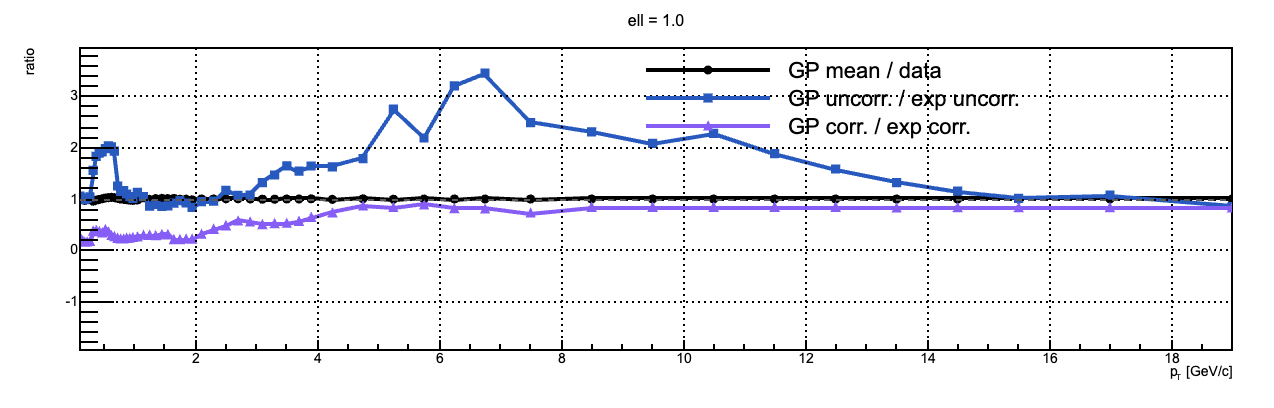
\includegraphics[width=0.9\textwidth]{img/Atlas-ell-1.0.png}
       \caption{GP fit: fixed ell = 1.0}
       \label{fig:results_model_validation_1}
   \end{figure}
\end{frame}

\begin{frame}{Results}
\frametitle{Atlas ins1759506 studies}
   \begin{figure}[h]
       \centering
       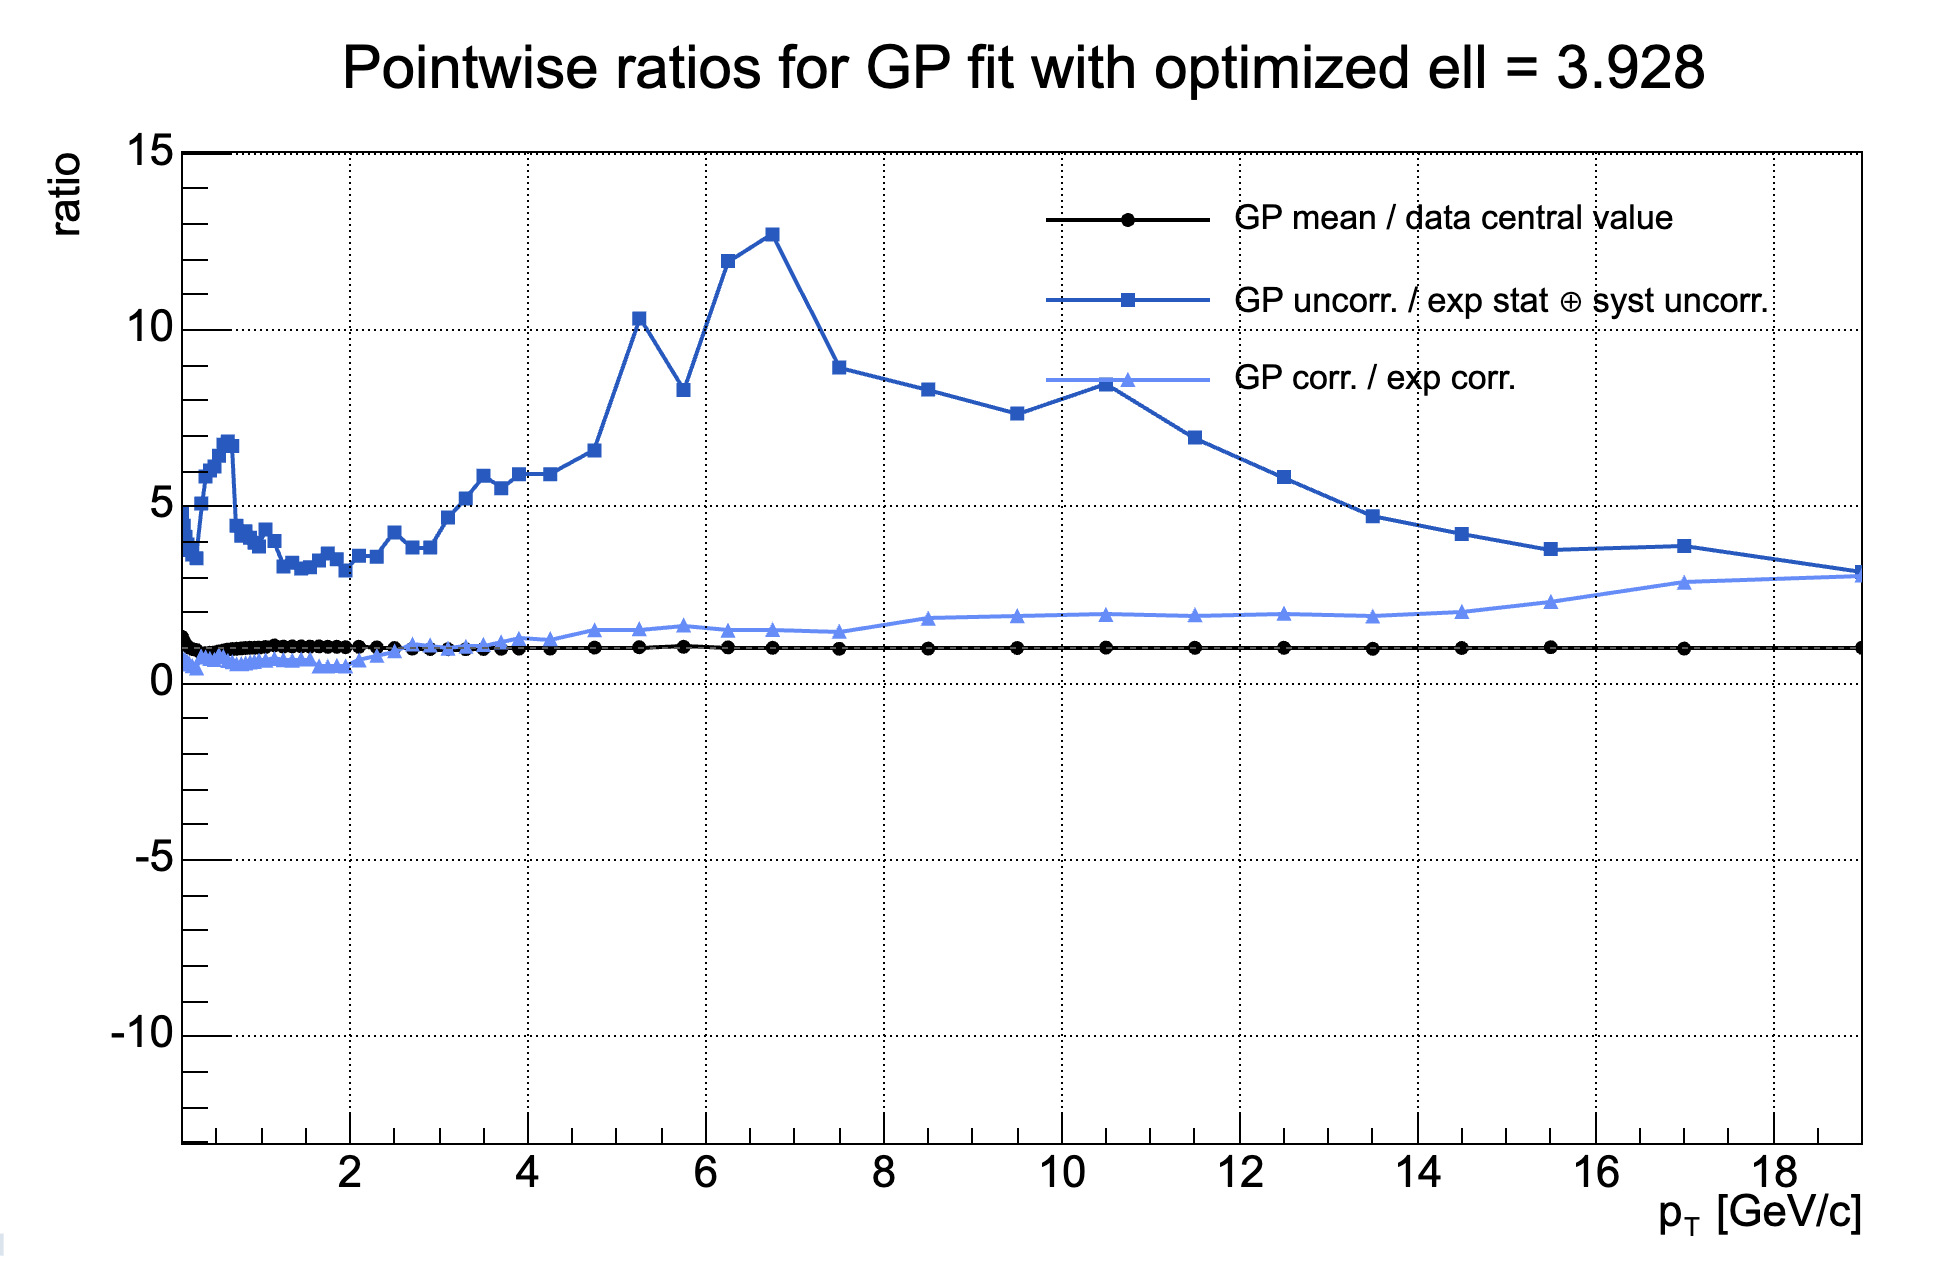
\includegraphics[width=0.7\textwidth]{img/Atlas-optimized_ell.png}
       \caption{GP fit: optimized ell}
       \label{fig:results_model_validation_2}
   \end{figure}
\end{frame}

\begin{frame}{Results}
\frametitle{Atlas ins1759506 studies}
   \begin{figure}[h]
       \centering
       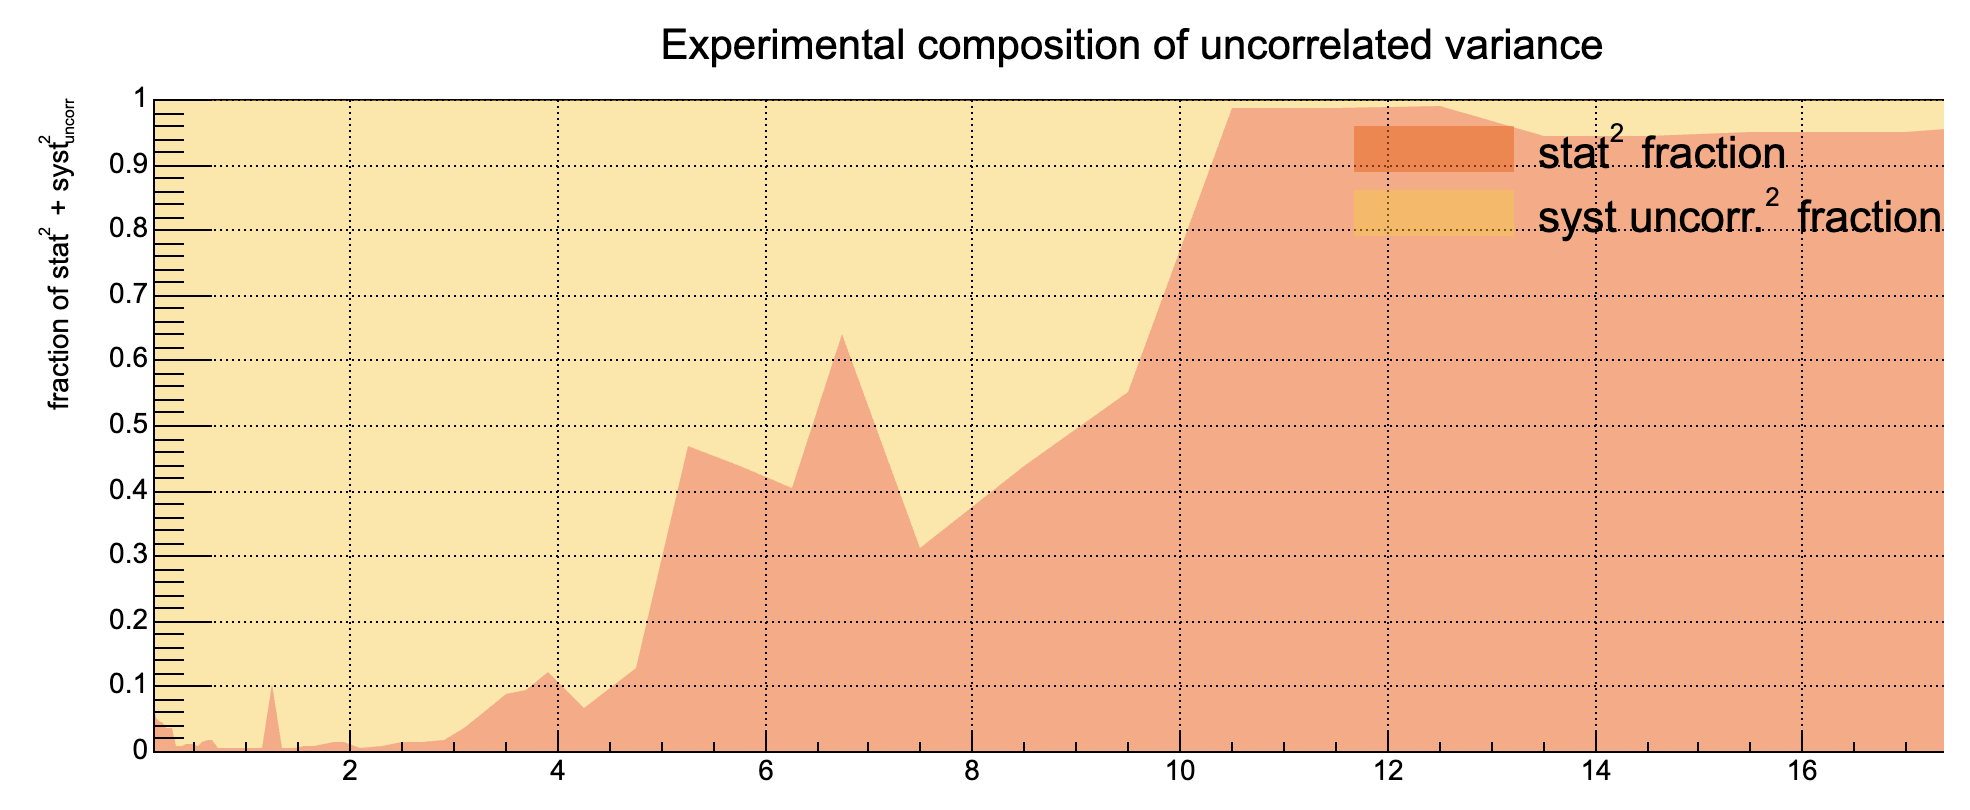
\includegraphics[width=0.9\textwidth]{img/Atlas-ratio.png}
       \caption{Ratio between white noise and systematic uncorrelated noise}
       \label{fig:results_posterior_predictive}
   \end{figure}
\end{frame}

\begin{frame}{Results}
\frametitle{Alice PbPb2760 Scaled Spectra studies}
   \begin{figure}[h]
       \centering
       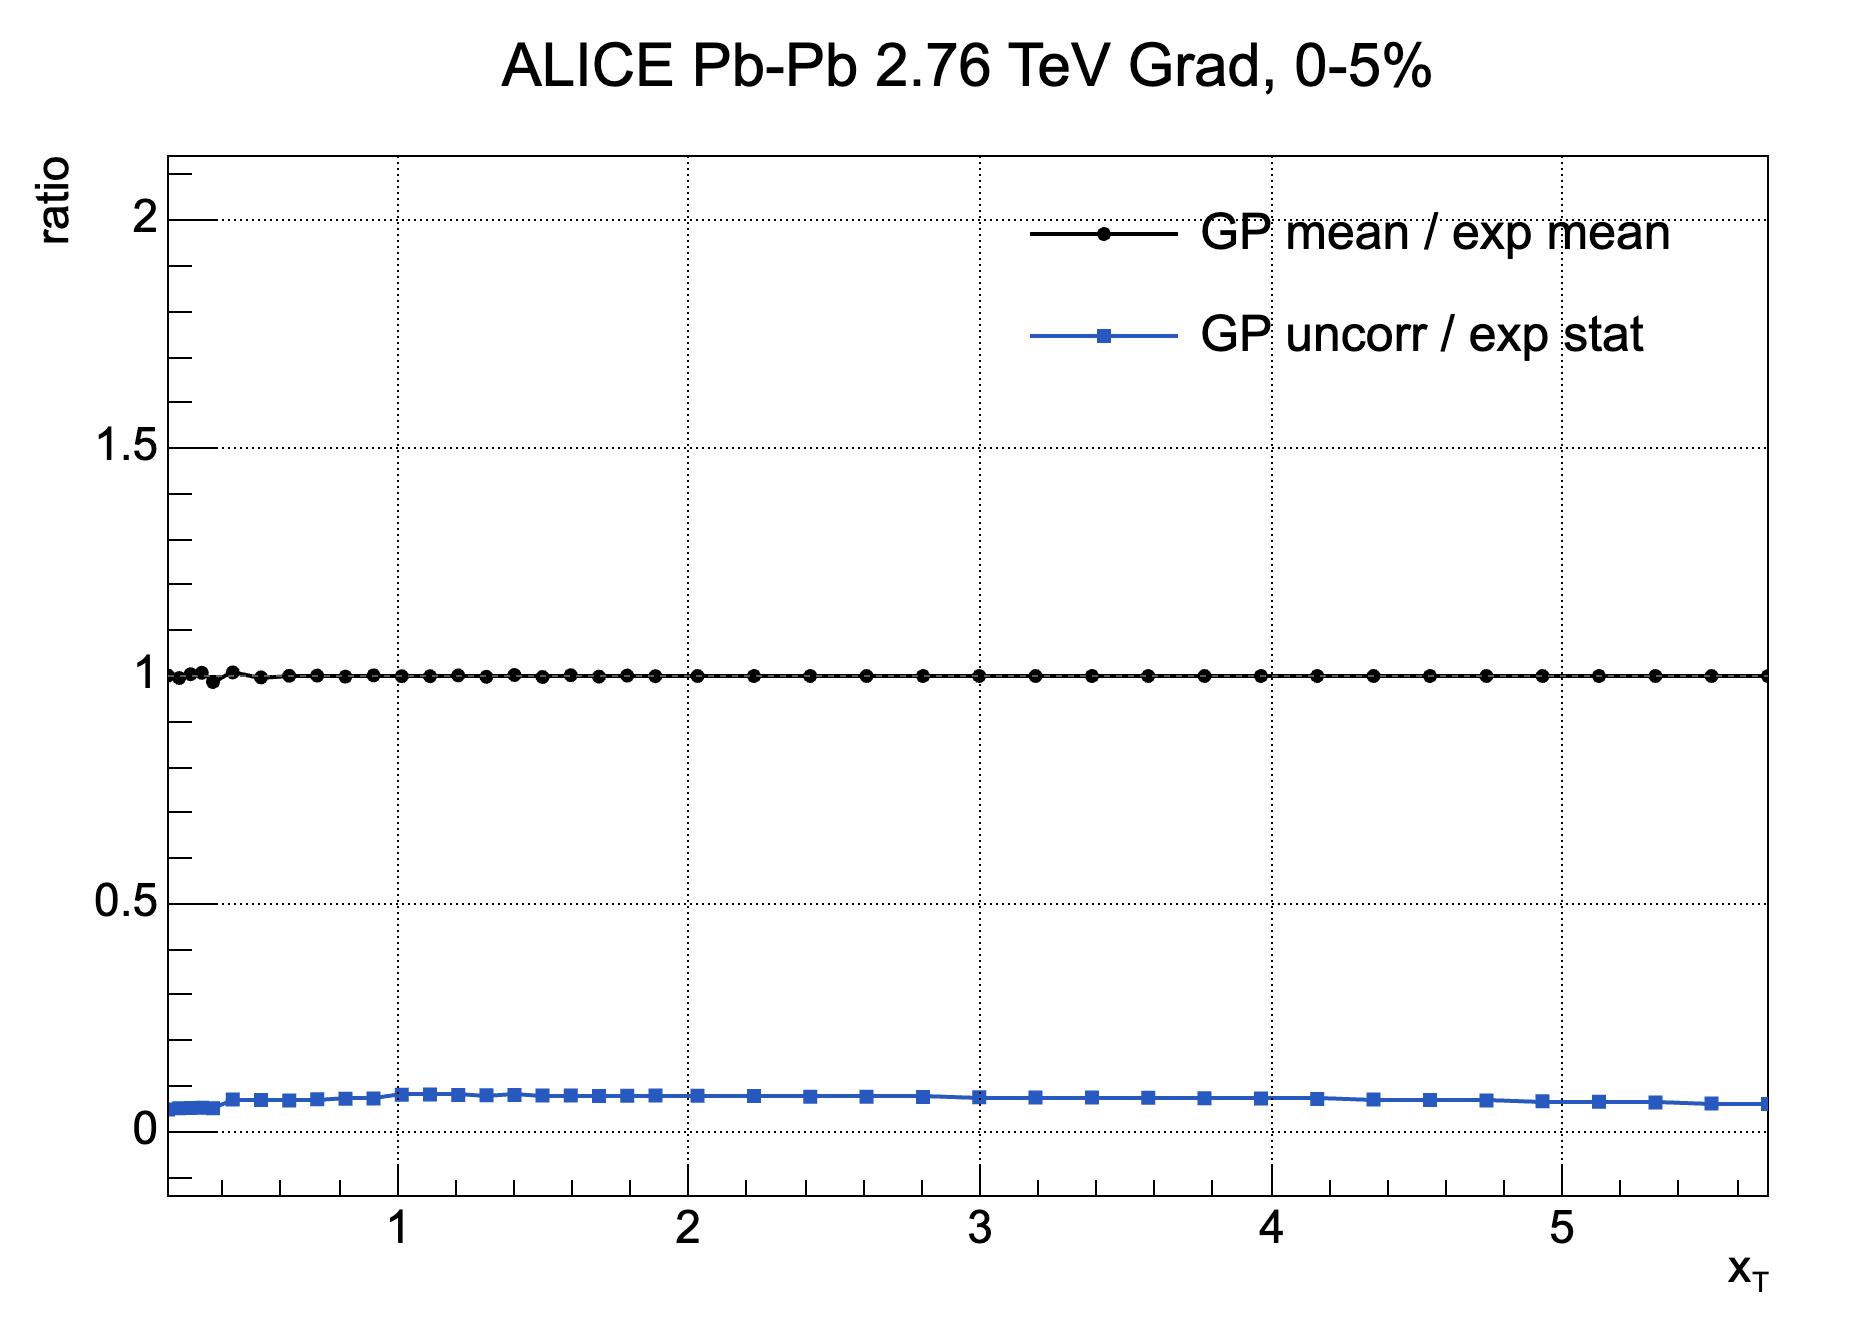
\includegraphics[width=0.7\textwidth]{img/Alice-ell-0.2.png}
       \caption{GP fit: fixed ell = 0.2}
       \label{fig:results_posterior_predictive}
   \end{figure}
\end{frame}

\begin{frame}{Results}
\frametitle{Alice PbPb2760 Scaled Spectra studies}
   \begin{figure}[h]
       \centering
       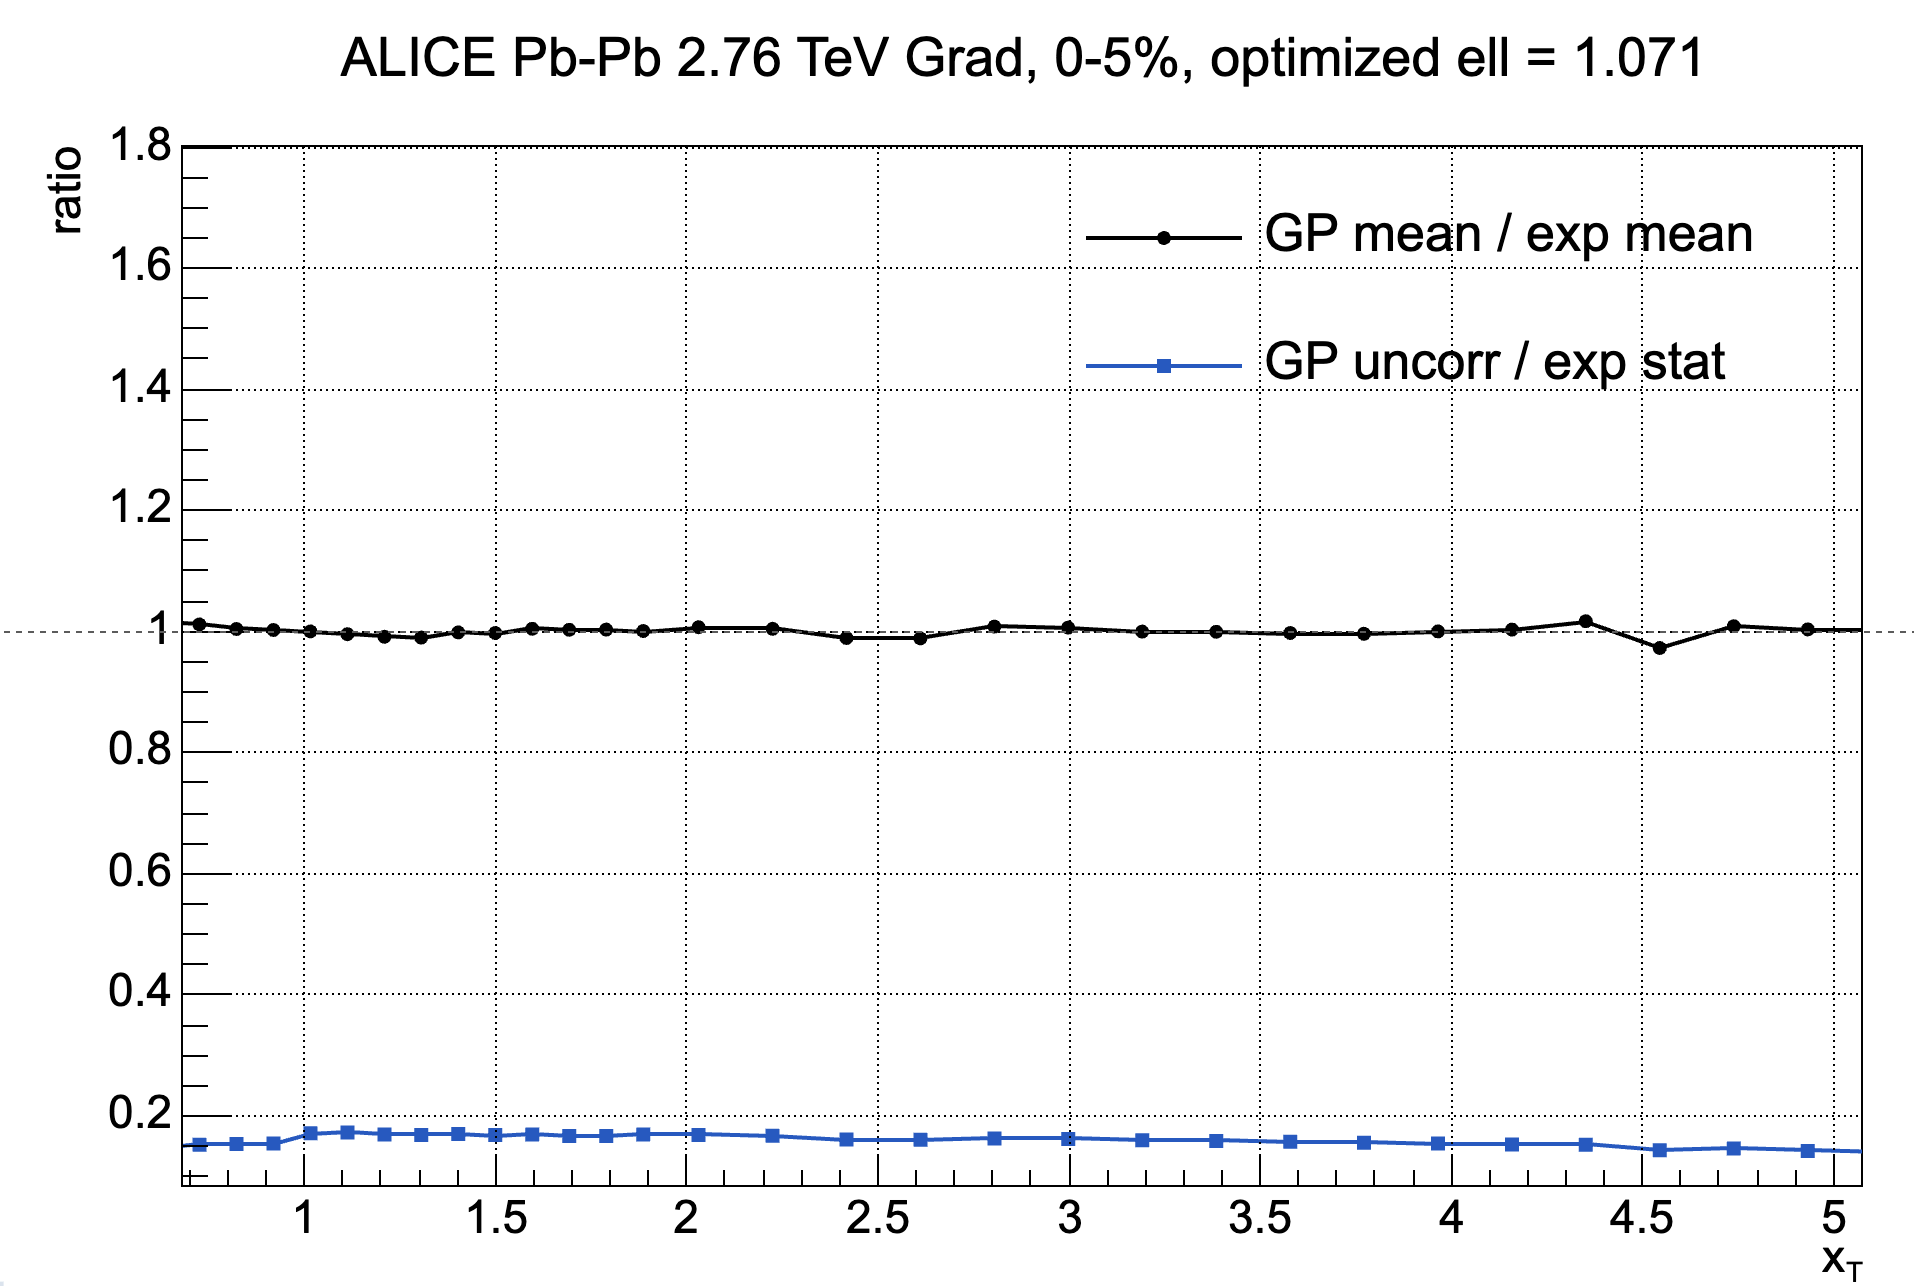
\includegraphics[width=0.7\textwidth]{img/Alice-Optimized_ell.png}
       \caption{GP fit: optimized ell}
       \label{fig:results_posterior_predictive}
   \end{figure}
\end{frame}

% \begin{frame}{Results}
% \frametitle{Preliminary results}
%    \begin{figure}[h]
%        \centering
%        
\includegraphics[width=0.5\textwidth]{img/corner_AuAu200_zeroexp_vs_baseline_vs_rho_0.9_vs_ro_10.0_Grad_1.png}
%        \caption{Preliminary results: Baseline vs zero correlation model vs $\rho=0.9$ vs $\rho=10.0$}
%        \label{fig:selected_article}
%    \end{figure}
% \end{frame}

% \begin{frame}{Results}
% \frametitle{Preliminary results}
%    \begin{figure}[h]
%        \centering
%        
\includegraphics[width=0.5\textwidth]{img/corner_AuAu200_zeroexp_vs_baseline_vs_rho_0.9_vs_ro_10.0_Grad_2.png}
%        \caption{Preliminary results: Baseline vs zero correlation model vs $\rho=0.9$ vs $\rho=10.0$}
%        \label{fig:selected_article}
%    \end{figure}
% \end{frame}
% \begin{frame}{Results}
% \frametitle{Baseline vs zero correlation model}
%    \begin{figure}[h]
%        \centering
%        
\includegraphics[width=0.5\textwidth]{img/corner_rho_0.9_Grad_2_vs_baseline_Grad_2_run_002_1.png}
%        \caption{}
%        \label{fig:selected_article}
%    \end{figure}
% \end{frame}

% \begin{frame}{Next Analysis}
% \frametitle{Next Analysis}
%    \begin{figure}[h]
%        \centering
%        
\includegraphics[width=0.5\textwidth]{img/image.png}
%        \caption{Mankolli, et al. JETSCAPE}
%        \label{fig:some_results}
%    \end{figure}
% \end{frame}

% \begin{frame}
%   \frametitle{Tasks Planned}
% \begin{table}[h]
% \centering
% \begin{tabular}{|l|c|}
% \hline
% \textbf{Task} & \textbf{Due Date} \\
% \hline
%   &  \\
% \hline
%   &  \\
% \hline
% \end{tabular}
% \end{table}
% \end{frame}
%----------------------------------------------------------------------------------------
% \begin{frame}[fragile]
%     \frametitle{Python}
    
%     \begin{python}
% def calcular_dobro(x):
%     """Retorna o dobro do número"""
%     return 2 * x

% # Testando a função
% numero = 5
% resultado = calcular_dobro(numero)
% print(f"O dobro de {numero} é {resultado}")
%     \end{python}
% \end{frame}

%----------------------------------------------------------------------------------------
% \begin{frame}[fragile]
%     \frametitle{C}
    
%     \begin{clang}
% #include <stdio.h>

% int main() {
%     int numero = 5;
%     int dobro = 2 * numero;
    
%     printf("O dobro de %d eh %d\n", numero, dobro);
%     return 0;
% }
%     \end{clang}
% \end{frame}

%----------------------------------------------------------------------------------------
% \begin{frame}[fragile]
%     \frametitle{C++}
    
%     \begin{cpp}
% #include <iostream>
% using namespace std;

% int main() {
%     int numero = 5;
%     int dobro = 2 * numero;
    
%     cout << "O dobro de " << numero;
%     cout << " eh " << dobro << endl;
%     return 0;
% }
%     \end{cpp}
% \end{frame}

%----------------------------------------------------------------------------------------
% \begin{frame}[fragile]
%     \frametitle{R}
    
%     \begin{rlang}
% # Função para calcular o dobro
% calcular_dobro <- function(x) {
%   return(2 * x)
% }

% # Testando a função
% numero <- 5
% resultado <- calcular_dobro(numero)
% print(paste("O dobro de", numero, "é", resultado))
%     \end{rlang}
% \end{frame}

%----------------------------------------------------------------------------------------

% \begin{frame}[fragile]
%     \frametitle{Java}
    
%     \begin{java}
% public class Exemplo {
%     public static void main(String[] args) {
%         int numero = 5;
%         int dobro = 2 * numero;
        
%         System.out.println("O dobro de " + numero +
%                          " eh " + dobro);
%     }
% }
%     \end{java}
% \end{frame}